\documentclass{article}
\usepackage[T1]{fontenc}
\usepackage{lmodern}
\usepackage{graphicx}
\usepackage{amsmath,amssymb}
\usepackage[a4paper,margin=2cm]{geometry}
\usepackage[absolute,overlay]{textpos}
\setlength{\TPHorizModule}{1mm}
\setlength{\TPVertModule}{1mm}
\usepackage[indonesian]{babel}
\usepackage{hyperref}
\setlength{\emergencystretch}{2em}
% unit: Halaman 50

\begin{document}

% === Halaman 50 (python/native) ===

Modern Cryptography

• Enkripsi dan dekripsi pesan dalam bentuk digital dengan komputer digital

50

50

1. Teks


2. Audio 


3. Gambar (image)

4. Video 


- DES, 3DES

- AES, Serpent

- RSA, ElGamal, ECC

- Diffie-Hellman

- MD5, SHA-3

- DSA

- TLS

- dll

% deskripsi: gambar native xref 247
\noindent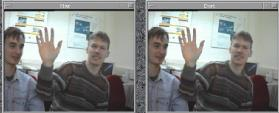
\includegraphics[width=0.85\textwidth]{../../images/python/page_050_img_01.jpeg}

% deskripsi: gambar native xref 248
\noindent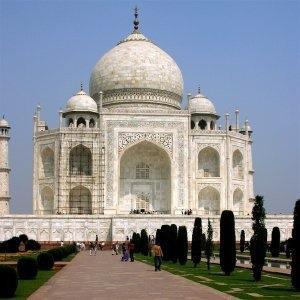
\includegraphics[width=0.85\textwidth]{../../images/python/page_050_img_02.jpeg}

% deskripsi: gambar native xref 249
\noindent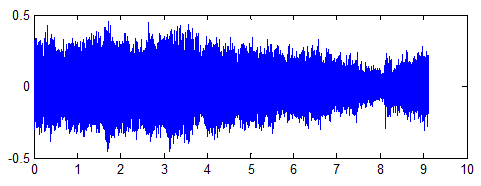
\includegraphics[width=0.85\textwidth]{../../images/python/page_050_img_03.png}

% deskripsi: gambar native xref 250
\noindent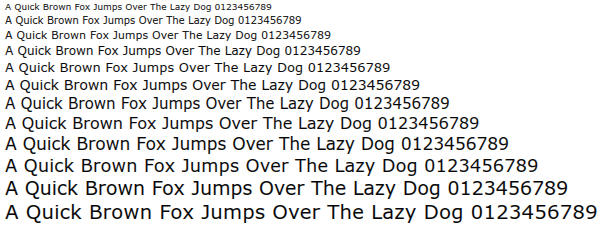
\includegraphics[width=0.85\textwidth]{../../images/python/page_050_img_04.png}

\end{document}
